
%%%%%%%%%%%%%%%%%%%%%%% file typeinst.tex %%%%%%%%%%%%%%%%%%%%%%%%%
%
% This is the LaTeX source for the instructions to authors using
% the LaTeX document class 'llncs.cls' for contributions to
% the Lecture Notes in Computer Sciences series.
% http://www.springer.com/lncs       Springer Heidelberg 2006/05/04
%
% It may be used as a template for your own input - copy it
% to a new file with a new name and use it as the basis
% for your article.
%
% NB: the document class 'llncs' has its own and detailed documentation, see
% ftp://ftp.springer.de/data/pubftp/pub/tex/latex/llncs/latex2e/llncsdoc.pdf
%
%%%%%%%%%%%%%%%%%%%%%%%%%%%%%%%%%%%%%%%%%%%%%%%%%%%%%%%%%%%%%%%%%%%


\documentclass[runningheads,a4paper]{llncs}

\usepackage{amssymb}
\setcounter{tocdepth}{3}
\usepackage{graphicx}
\usepackage{multirow}
\usepackage{subfigure}
\usepackage{graphics}

\usepackage{rotating}
\usepackage{verbatim}
\usepackage{float}


\usepackage{url}
\urldef{\mailsa}\path|{alfred.hofmann, ursula.barth, ingrid.haas, frank.holzwarth,|
\urldef{\mailsb}\path|anna.kramer, leonie.kunz, christine.reiss, nicole.sator,|
\urldef{\mailsc}\path|erika.siebert-cole, peter.strasser, lncs}@springer.com|    
\newcommand{\keywords}[1]{\par\addvspace\baselineskip
\noindent\keywordname\enspace\ignorespaces#1}

\usepackage{listings}
\usepackage{color}
\definecolor{javared}{rgb}{0.6,0,0} % for strings
\definecolor{javagreen}{rgb}{0.25,0.5,0.35} % comments
\definecolor{javapurple}{rgb}{0.5,0,0.35} % keywords
\definecolor{javadocblue}{rgb}{0.25,0.35,0.75} % javadoc
 
\lstset{language=Java,
basicstyle=\ttfamily,
keywordstyle=\color{javapurple}\bfseries,
stringstyle=\color{javared},
commentstyle=\color{javagreen},
morecomment=[s][\color{javadocblue}]{/**}{*/},
%numbers=left,
numberstyle=\tiny\color{black},
stepnumber=2,
numbersep=10pt,
tabsize=4,
showspaces=false,
showstringspaces=false}




\begin{document}

\mainmatter  % start of an individual contribution

% first the title is needed
\title{Automated Discovery of Failure Domain}

% a short form should be given in case it is too long for the running head
\titlerunning{Automated Discovery of Failure Domain}

% the name(s) of the author(s) follow(s) next
%
% NB: Chinese authors should write their first names(s) in front of
% their surnames. This ensures that the names appear correctly in
% the running heads and the author index.
%
\author{Mian Ahmad%
%\thanks{Please note that the LNCS Editorial assumes that all authors have usedn the western naming convention, with given names preceding surnames. This determines the structure of the names in the running heads and the author index.}%
\and Manuel Oriol}
%
\authorrunning{Automated Discovery of Failure Domain} %: Authors' Instructions}
% (feature abused for this document to repeat the title also on left hand pages)

% the affiliations are given next; don't give your e-mail address
% unless you accept that it will be published
\institute{University of York, Department of Computer Science,\\
Deramore Lane, YO10 5GH YORK, United Kingdom\\
%\mailsa\\
%\mailsb\\
%\mailsc\\
%\url{http://www.springer.com/lncs}}
}

%
% NB: a more complex sample for affiliations and the mapping to the
% corresponding authors can be found in the file "llncs.dem"
% (search for the string "\mainmatter" where a contribution starts).
% "llncs.dem" accompanies the document class "llncs.cls".
%

\toctitle{Lecture Notes in Computer Science}
\tocauthor{Authors' Instructions}
\maketitle


\begin{abstract}
There are several automated random strategies of software testing based on the presence of point, block and strip fault domains inside the whole input domain. As yet no particular, fully automated test strategy has been developed for the discovery and evaluation of the fault domains. We therefore have developed Automated Discovery of Failure Domain, a new random test strategy that finds the faults and the fault domains in a given system under test. It further provides visualisation of the identified pass and fail domain. In this paper we describe ADFD strategy, its implementation in YETI and illustrate its working with the help of an example. We report on experiments in which we tested error seeded one and two-dimensional numerical programs. Our experimental results show that for each SUT, ADFD strategy successfully performs identification of faults, fault domains and their representation on graphical chart.


%The abstract should summarize the contents of the paper and shouldcontain at least 70 and at most 150 words. It should be written using the \emph{abstract} environment.
%\keywords{We would like to encourage you to list your keywords within the abstract section}
\keywords{automated, software, testing, random, YETI, failure domain, point, block, strip}

\end{abstract}





\section{Introduction}\label{sec:intro}

Testing is fundamental requirement to assess the quality of any software. Manual testing is labour-intensive and error-prone; therefore emphasis is to use automated testing that significantly reduces the cost of software development process and its maintenance \cite{Beizer1995}. Most of the modern black-box testing techniques execute the System Under Test (SUT) with specific input and compare the obtained results against the test oracle. A report is generated at the end of each test session containing any discovered faults and the input values which triggers the faults. Debuggers fix the discovered faults in the SUT with the help of these reports. The revised version of the system is given back to the testers to find more faults and this process continues till the desired level of quality, set in test plan, is achieved.

The fact that exhaustive testing for any non-trivial program is impossible, compels the testers to come up with some strategy of input selection from the whole input domain. Pure random is one of the possible strategies widely used in automated tools. It is intuitively simple and easy to implement \cite{Ciupa2008},  \cite{Forrester2000}. It involves minimum or no overhead in input selection and lacks human bias \cite{Hamlet1994},  \cite{Linger1993}. While pure random testing has many benefits, there are some limitations as well, including low code coverage \cite{Offutt1996} and discovery of lower number of faults \cite{Chen1994}. To overcome these limitations while keeping its benefits intact many researchers successfully refined pure random testing. Adaptive Random Testing (ART) is the most significant refinements of random testing. Experiments performed using ART showed up to 50\% better results compared to the traditional/pure random testing  \cite{Chen2008}.  Similarly Restricted Random Testing (RRT) \cite{Chan2002}, Mirror Adaptive Random Testing (MART)  \cite{Chen2004}, Adaptive Random Testing for Object Oriented Programs (ARTOO) \cite{Ciupa2008}, Directed Adaptive Random Testing (DART)  \cite{Godefroid2005}, Lattice-based Adaptive Random Testing (LART) \cite{Mayer2005} and Feedback-directed Random Testing (FRT) \cite{Pacheco2007} are some of the variations of random testing aiming to increase the overall performance of pure random testing.

All the above-mentioned variations in random testing are based on the observation of Chan et. al.,  \cite{Chan1996} that failure causing inputs across the whole input domain form certain kinds of domains. They classified these domains into point, block and strip fault domain. In Figure \ref{fig:patterns} the square box represents the whole input domain. The black point, block and strip area inside the box represent the faulty values while white area inside the box represent legitimate values for a specific system. They further suggested that the fault finding ability of testing could be improved by taking into consideration these failure domains.

\begin{figure}[h]
 \centering
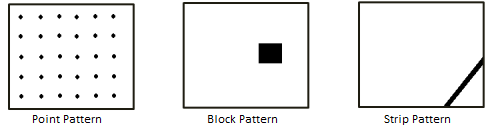
\includegraphics[width=8cm,height=2cm]{ART_Patterns.png}
\caption{Failure domains across input domain \cite{Chan1996}}
\label{fig:patterns}
\end{figure}


% It is important to note that these techniques only identify a single instance of failure and do not  focus on the failure domain. 

%2.	It is also noticed that further analysis of fault lead to new faults which the testing process may not have identified.
%3. 	Experiments can be performed to analyse the frequency of existence of point, block and strip domain across the input domain. 

%Random testing is a black-box testing technique in which parts (methods/modules) of SUT are selected randomly and then executed against randomly generated test data from the whole input domain. Results obtained from the execution are either compared to the specifications of the SUT or language exceptions which served as a test oracle. Any test output that fail to meet the oracle either because of failing to comply the specification or trigger the exceptions are considered as potential faults. In this paper we present a new tool, called Automated Discovery of Failure Domain (ADFD), based on a random testing tool called York Extensible Testing Infrastructure (YETI), for not only finding fault but also its domain. ADFD utilise YETI to discover the fault in the given SUT and then generate a dynamic code for finding its domain. The found domain -- point, block or strip are presented on the graph at the end of each test session


%ADFD has been designed to decrease the time of system testing. Knowing the domain of the fault the debuggers This research can decrease the overall testing time by reducing the number of code exchanges between testers and debugger. It is achieved by tracking the failure domain and not only a single instance failure. Tracking failure domain provide more information about the behaviour of the fault.

%that also served as regression testing. None of the testing techniques evaluate the nature of the fault and the pattern in which the fault reside. 


%The aim of this research study is to find not only find the values for which the system fails but also the domains of failure causing inputs which will help in automated generation of fault targeted test cases for any black-box testing technique.\\


%Over the past few years there is a tremendous growth in development of hardware whose main focus is to increase the computer processing power. The computers that served as a mini and mainframe computers few years ago are turned into personal computer in todays modern age. To utilise this processing power various software development companies started to develop more sophisticated and processing hungry softwares. These softwares provide simple and easy to use Graphical User Interface (GUI) but on the back end they are equally complex and consist of thousands of instructions. This increase in size of the software also increases the difficulty of preserving high quality, reliability, portability, maintainability and efficiency of the software. These problems are mainly cater by software testing. The increase of complexity and size of softwares also forced the researchers to find new ways of software testing that are more efficient, reliable and speedy to cope with the ever increasing hardware and software industry.\\

%Mirror Adaptive Random Testing (MART)  \cite{Chen2003}, Feedback-directed Random Testing (FDRT) \cite{Pacheco2007}, Restricted Random Testing (RRT) \cite{Chan2002} and Quasi Random Testing  (QRT) \cite{Chen2005} are the strategies based on the same principle that found better results compared to ordinary random testing.

It is interesting that where many random strategies are based on the principle of contiguous fault domains inside the input domain, no specific strategy is developed to evaluate these fault domains. This paper describes a new test strategy called Automated Discovery of Failure Domain (ADFD), which not only finds the pass and fail input values but also finds their domains. The idea of identification of pass and fail domain is attractive as it provides an insight of the domains in the given SUT. Some important aspects of ADFD strategy presented in the paper include:

\begin{itemize}
\item Implementation of the new ADFD strategy in York Extensible Testing Infrastructure (YETI) tool.
\item Evaluation to assess ADFD strategy by testing classes with different fault domains.
\item Decrease in overall test duration by identification of all the fault domains instead of a single instance of fault.
\item Increase in test efficiency by helping debugger to keep in view all the fault occurrences when debugging. 
\end{itemize}


% Additionally, ADFD test strategy can also be used to identify frequency of point, block and strip fault domain across the production softwares.



%The main objective behind ADFD is to get an automated frame work that find the existence of fault and fault domain across the input domain, decrease debugging time and to discover any more faults missed by the testing system. Significant research has been done to utilise the failure domains but their existence, nature and boundaries need further attention. Having fault domain information prior to testing enables the tester to guide testing according to the failure domain of the SUT, for example pure random testing is more effective for point domain than block and strip domains where as ART, MART, FDRT, RRT and QRT are more effective for block and strip fault domains than point fault domain.

%In our previous research we extended the same idea of the existence of different domains of failure across the whole input domain proposed by Chen et al, \cite{Chen2008} and accepted by various other researchers to develop a new strategy called Dirt Spot Sweeping Strategy [X]. However the experimental results showed not very considerable improvement then what we predicted. We performed 500 experiments in which we carried out 10000 tests but the results showed only 5\% improvement contrary to our prediction of 30\%. All the experiments were performed from a pool of open-source projects bundled in a repository called Qualitas Corpus \cite{Tempero2010}. Corpus contains more than 100 open-source java projects and maintained only for the purpose of unbiased research experiments. Therefore one of the conclusions derived from our experiments was that the patterns of failure may not exist in most of the software’s due to which our strategy which focus on these patterns didn’t produce much efficiency.\\
%It was therefore very interesting for us to do further research to find about the existence and nature of these failure patterns. Our main focus in this research paper is to discover whether there exist failure patterns across the input domain or not and if they exist then how frequent and what pattern they follow.\\

The rest of this paper is organized as follows: \\ Section~\ref{sec:adfd} describes the ADFD strategy. Section~\ref{sec:implementation} presents implementation of the ADFD strategy. Section~\ref{sec:experimentalResults} explains the experimental results. Section~\ref{sec:discussion} discusses the results. Section~\ref{sec:validity} presents the threats to validity. Section~\ref{sec:relatedWork} presents related work and Section~\ref{sec:conclusion}, concludes the study.

%In Section II, we describe the automated discovery of failure domain test strategy and explain its structure and function with the help of a flowchart and motivating example. Section III presents its implementation in automated random testing tool called York Extensible Testing Infrastructure (YETI). Section IV and V report the experiments performed using the proposed technique and evaluate \& discuss the obtained results. Section VI and VII discuss any threats to validity and related discussion. Finally we conclude in Section VIII. 

%The rest of this paper is organized as follows. The sections, II to X, describe automated strategy, Implementation, Experimental setup and analysis, Evaluation, Experimental results, discussion, conclusion and future work respectively.\\

%X\section{Problems and Solutions}\label{sec:probl_and_sol}
%This paper address five. main problems in random testing. These are (1) Finding the whole domain of fault instead of only failing values, (2) Representation of fault values, (3) automation of the evaluation process, (4) Identification of fault domain for multi arguments methods and its representation, (5) Generation and classification of test values for Strings and complex (non scaler) arguments. This section elaborate each of the above mention problem and describe our proposed solution (if any) to them.

%\subsection{Finding the whole domain of fault instead of only failing values}
%Most of the testing tools take into account only the fault finding values with out giving due consideration to the domain in which the values exist. \subsection{Representation of fault values and fault domains}
%points: instead of dumping logs and more complex reports we describe the fault domains with the help of charts. 
%\subsection{Automation of the testing process}
%We developed an automated system to test the system, generate the fault domain finding files, compile and execute them to find the fault domains if any. points: automation is achieved by combining the test tool and evaluation system e.g. yeti and ADFD.   
%\subsection{Identification and representation of multi arguments data}
%I think it is beyond the scope of this study to identify and represent more then 3 arguments method because at the moment we can show only three diminutional charts.
%\subsection{Generation and classification of test values for string and complex (non scaler) arguments}
%It is difficult to find the domain for strings and complex (non scaler) data therefore they can be exempted from this study.


\section{Automated Discovery of Failure Domain}\label{sec:adfd}

Automated Discovery of Failure Domain (ADFD) strategy is proposed as improvement on R+ strategy with capability of finding faults as well as the fault domains. The output produced at the end of test session is a chart showing the passing value or range of values in green and failing value or range of values in red. The complete workflow of ADFD strategy is given in Figure \ref{fig:ADFD}.

The process is divided into five major steps given below and each step is briefly explained in the following paras.

\begin{enumerate}
\item GUI front-end for providing input
\item Automated finding of fault
\item Automated generation of modules
\item Automated compilation and execution of modules to discover domains
\item Automated generation of graph showing domains
\end{enumerate}

\begin{figure}[ht]
\centering
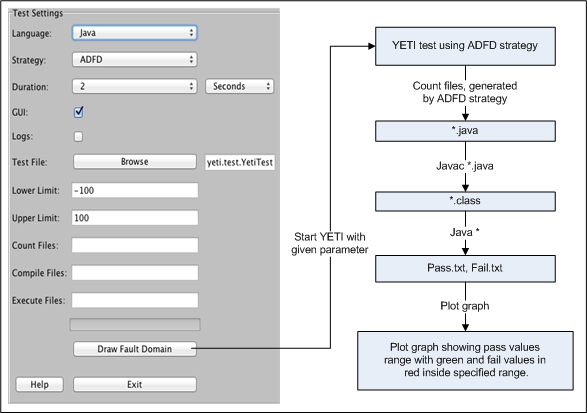
\includegraphics[width=8.2cm,height=6cm]{ADFD-Diagram1.png}
\caption{Work flow of ADFD strategy}
\label{fig:ADFD}
\end{figure}

\begin{figure}[htp]
\begin{center}
%\centring
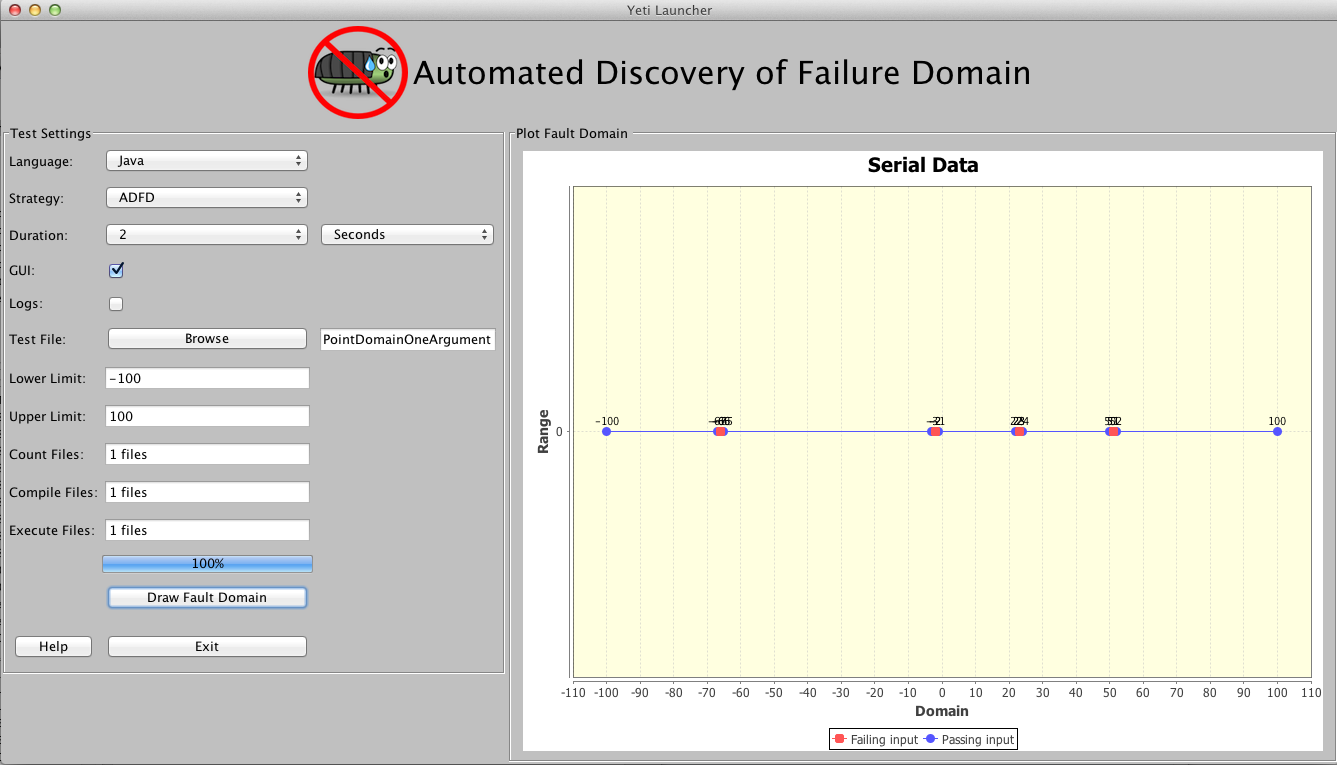
\includegraphics[width=12cm,height=6.6cm]{ADFD-front-end.png}
\caption{Front-end of ADFD strategy}
\label{fig:ADFD}
\end{center}
\end{figure}

\noindent \textbf{GUI front-end for providing input:}\\*
\indent ADFD strategy is provided with an easy to use GUI front-end to get input from the user. It takes YETI specific input including language of the program, strategy, duration, enable or disable YETI GUI, logs and a program to test in the form of java byte code. In addition it also takes minimum and maximum values to search for fault domain in the specified range. Default range for minimum and maximum is Integer.MIN\_INT and Integer.MAX\_INT respectively.\\

\noindent \textbf{Automated finding of fault:}\\*
\indent To find the failure domain for a specific fault, the first requirement is to identify that fault in the system. ADFD strategy extends R+ strategy and rely on R+ strategy to find the first fault. Random+ (R+) is an improvement over random strategy with preference to the boundary values to provide better fault finding ability. ADFD strategy is implemented in YETI tool which is famous for its simplicity, high speed and proven ability of finding potentially hazardous faults in many systems \cite{Oriol2011},  \cite{Oriol2012}. YETI is quick and can call up to one million instructions in one second on Java code. It is also capable of testing VB.Net, C, JML and CoFoJa beside Java. \\

\noindent \textbf{Automated generation of modules:}\\*
\indent  After a fault is found in the SUT, ADFD strategy generate complete new Java program to search for fault domains in the given SUT.  These programs with ``.java" extensions are generated through dynamic compiler API included in Java 6 under javax.tools package. The number of programs generated can be one or more, depending on the number of arguments in the test module i.e. for module with one argument one program is generated, for two argument two programs and so on. To track fault domain the program keeps one or more than one argument constant and only one argument variable in the generated program.\\

\noindent \textbf{Automated compilation and execution of modules to discover domains:}\\*
\indent  The java modules generated in previous step are compiled using ``javac *" command to get their binary ``.class" files. The ``java *" command is applied to execute the compiled programs. During execution the constant arguments of the module remain the same but the variable argument receive all the values in range, from minimum to maximum, specified in the beginning of the test. After execution is completed we get two text files of ``Pass.txt" and ``Fail.txt". Pass file contains all the values for which the modules behave correctly while fail file contains all the values for which the modules fail.\\

\noindent \textbf{Automated generation of graph showing domains:}\\*
\indent The values from the pass and fail files are used to plot (x, y) chart using JFreeChart. JFreeChart is a free open-source java library that helps developers to display complex charts and graphs in their applications \cite{Gilbert2008}. Green colour lines with circle represents pass values while red colour line with squares represents the fail values. Resultant graph clearly depicts both the pass and fail domain across the specified input domain. The graph shows red points in case the program fails for only one value, blocks when the program fails for multiple values and strips when a program fails for a long range of values.%\subsection{Flow Chart of the process}

%The following flow chart clearly identify the workflow of the whole process and the various steps involved in the process.

%\begin{figure}[p]
%\centering
%\includegraphics[width=8cm,height=12cm]{automatedFail.png}
%\caption{Automated discovery of Failure Domain}
%\label{fig:autofail}
%\end{figure}




%We found that it is better for the developer to see the range because the fault can be found once but it can generate errors at multiple locations.like point pattern in the first graph only generate fault at location 0 but if the same zero is assigned to second argument then the whole domain values can fail.\\


%\begin{figure}[htp]
%\centering
%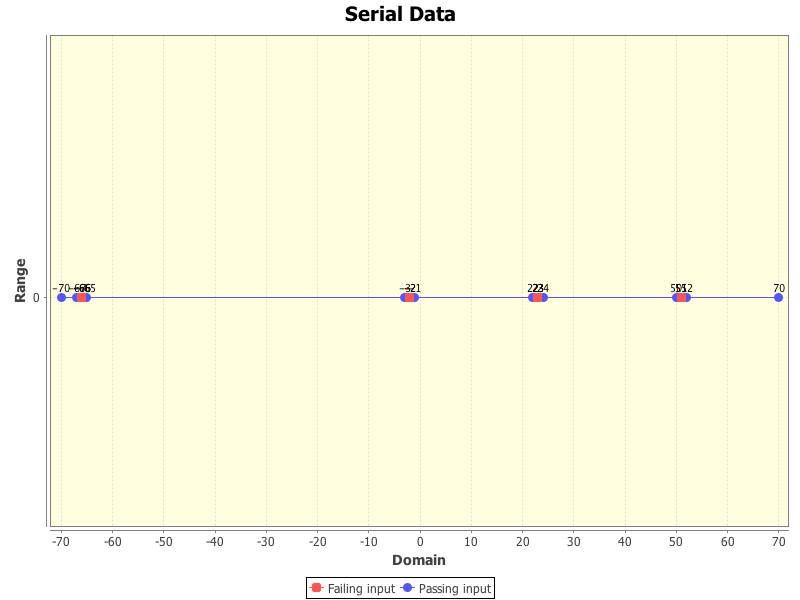
\includegraphics[width=8.5cm,height=6cm]{oneArgumentPointDomain.png}
%\caption{Point pattern failure domain}
%\label{fig:patterns}
%\end{figure}


%Figure \ref{fig:point} shows the example of point pattern. In sub figure \ref{fig1:a} test only fails for 0 out of the whole integer range where as in sub figure \ref{fig1:b} all test fails when static variable is assigned with 0 value.


%\begin{figure}[htp]
%\centering
%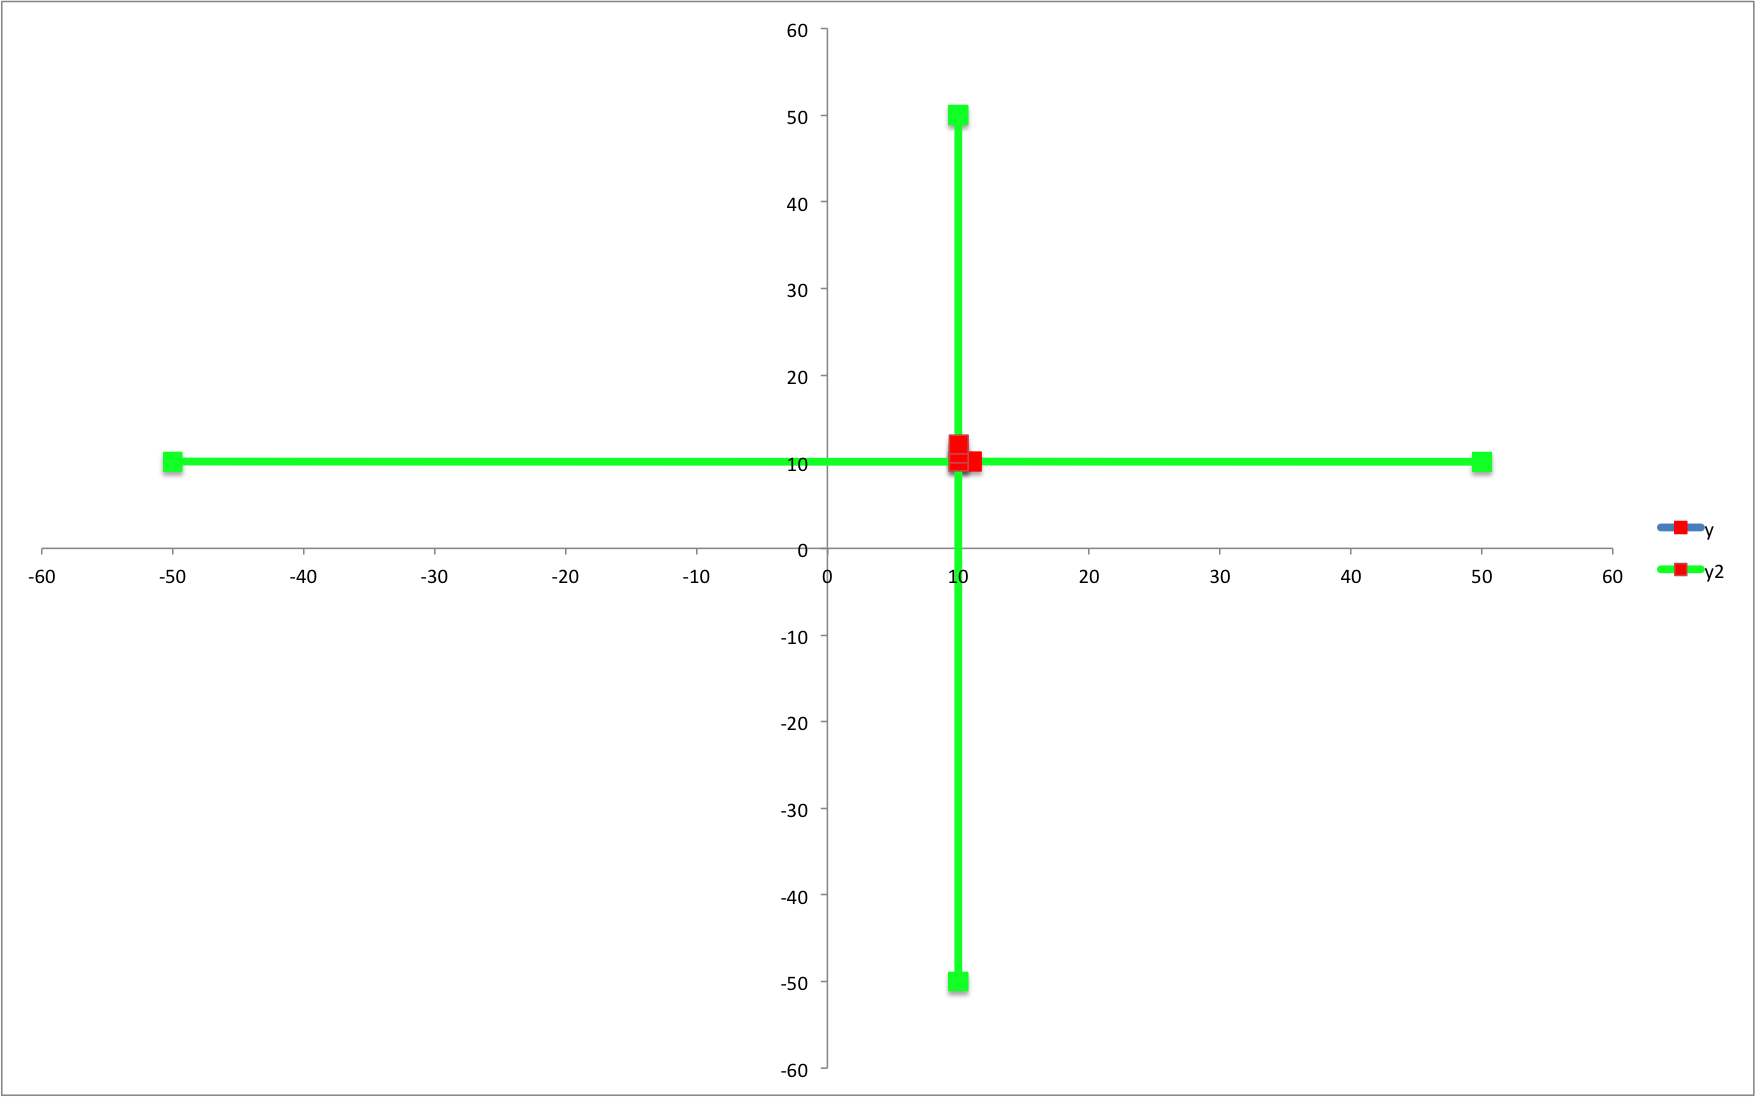
\includegraphics[width=4cm,height=4cm]{block_pattern.png}
%\caption{Block pattern failure domain}
%\label{fig:patterns}
%\end{figure}


%Figure \ref{fig:block} shows the example of block pattern. Both sub figure \ref{fig1:a} and \ref{fig1:b} shows the block pattern of failure. The failure values are given in table \ref{tb:failtable}.

%\begin{figure}[htp]
%\centering
%\begin{center}
%  % Maximum length
 %\subfloat[Test 1 A]{\label{fig1:a}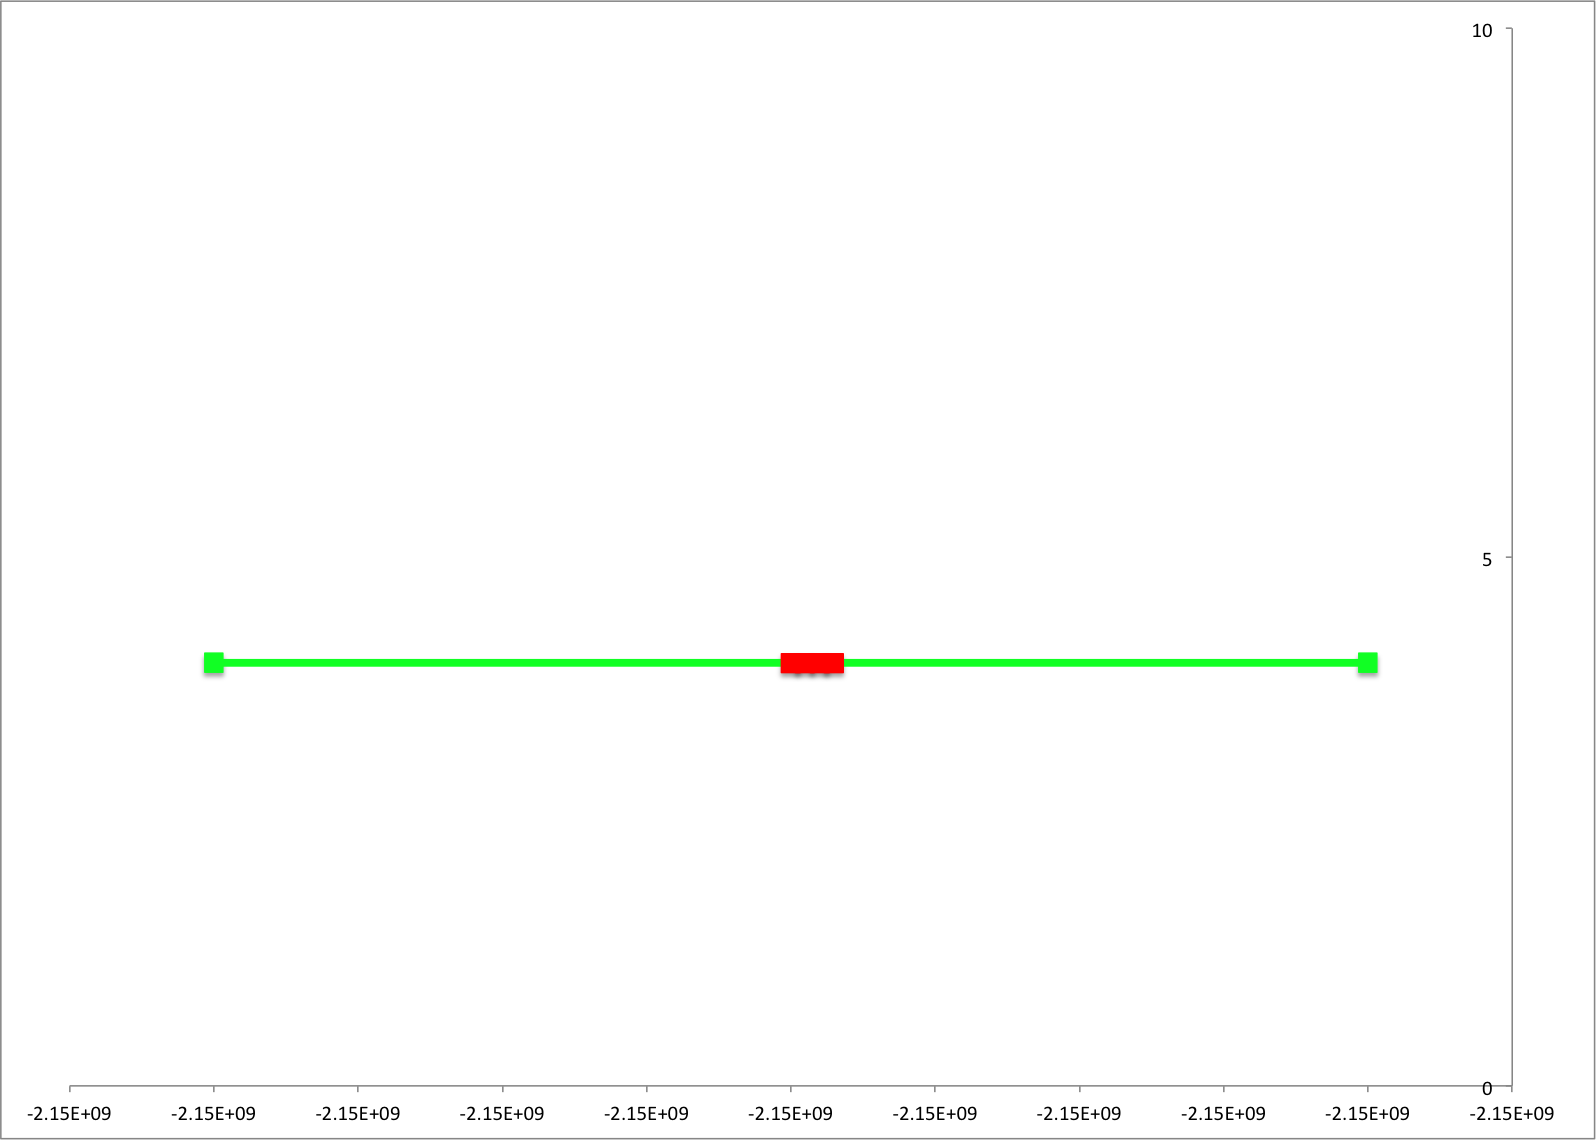
\includegraphics[width=0.49\linewidth]{excel_png/strip_pattern_B.png}}\hfill
 %\subfloat[Test 1 B]{\label{fig1:b}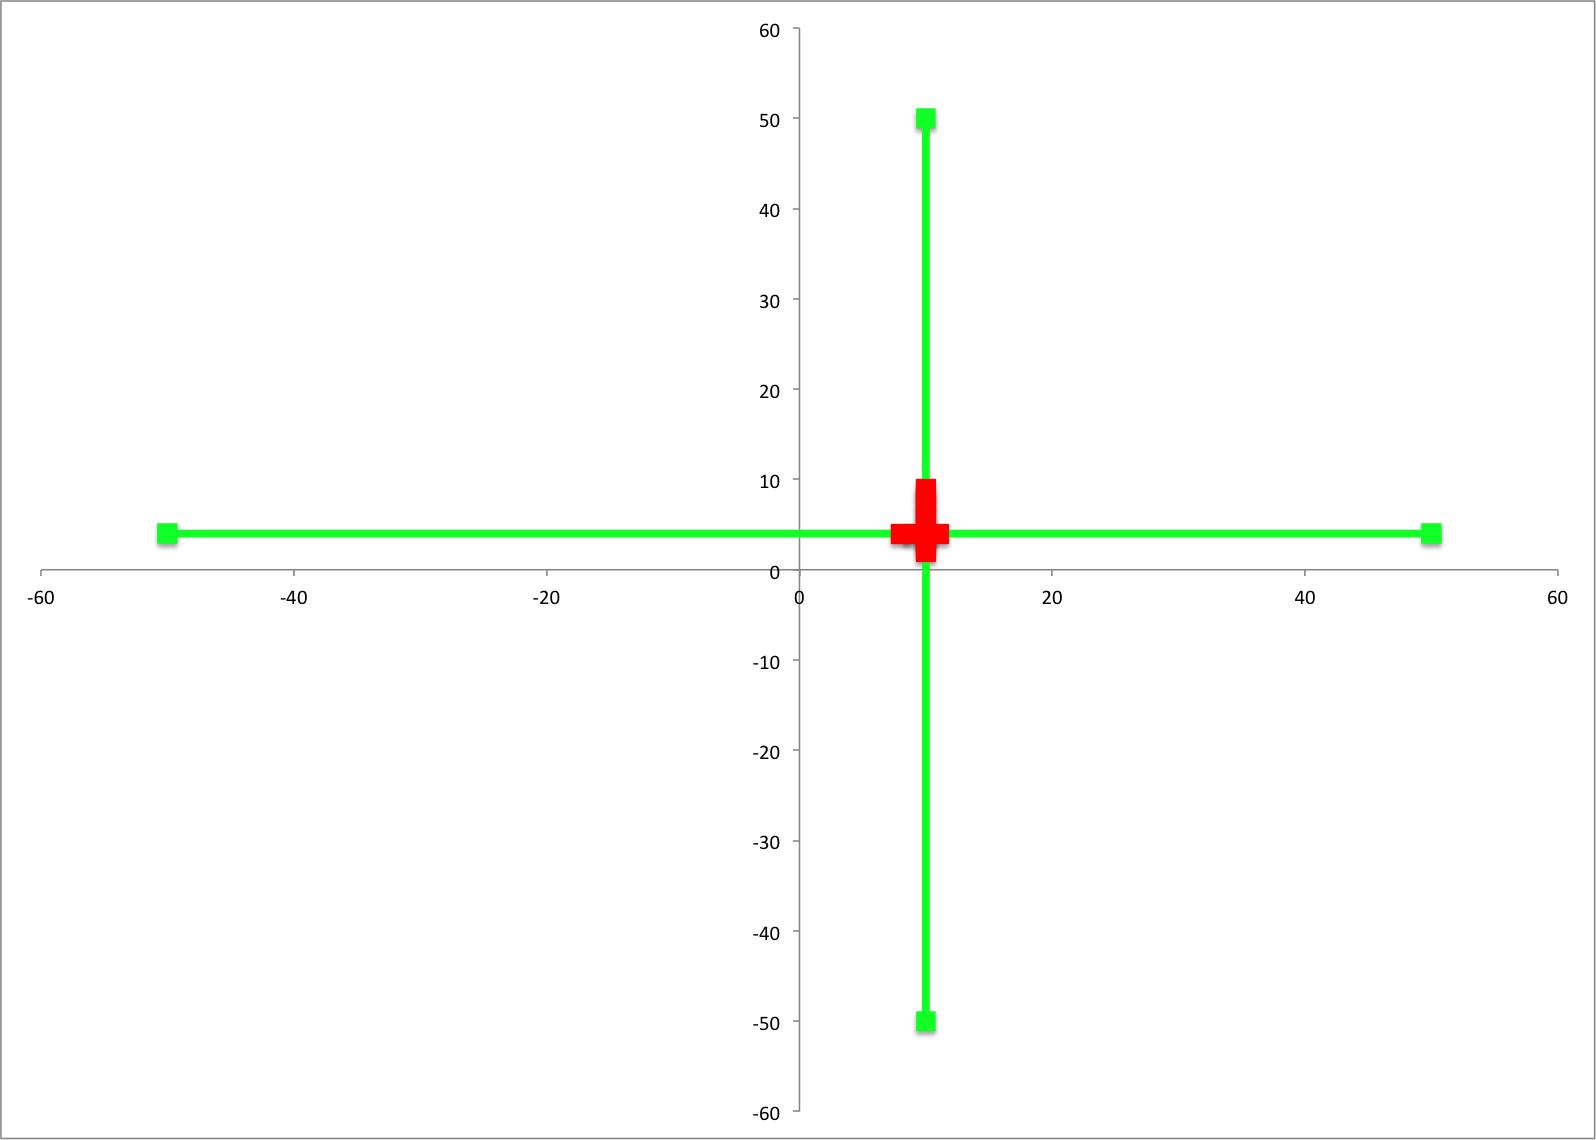
\includegraphics[width=0.49\linewidth]{excel_png/strip_pattern_A.png}}
%  end{center}
%\caption{Strip pattern failure domain}
%%  \label{fig:strip}
%\end{figure}

%Figure shows the example of strip pattern. Here we have two strip failure pattern for test 1 shown in \ref{fig1:a} and \ref{fig1:b} while 1 other for test 2 given in . The failure values are given in table .\\

\section{Implementation}\label{sec:implementation}
The ADFD strategy is implemented in a tool called York Extensible Testing Infrastructure (YETI). YETI is available in open-source at \url{http://code.google.com/p/yeti-test/}. In this section a brief overview of YETI is given with the focus on the parts relevant to the implementation of ADFD strategy. For integration of ADFD strategy in YETI, a program is used as an example to illustrate the working of ADFD strategy. Please refer to  \cite{Oriol2011},  \cite{Oriol2012}, \cite{Oriol2010},  \cite{Oriol2010a},  \cite{Oriol2010b} for more details on YETI tool.

 \subsection{York Extensible Testing Infrastructure}
YETI is a testing tool developed in Java that test programs using random strategies in an automated fashion. YETI meta-model is language-agnostic which enables it to test programs written in functional, procedural and object-oriented languages.

YETI consists of three main parts including core infrastructure for extendibility through specialisation, strategies section for adjustment of multiple strategies and languages section for supporting multiple languages. Both the languages and strategies sections have a pluggable architecture to easily incorporate new strategies and languages making YETI a favourable choice to implement ADFD strategy. YETI is also capable of generating test cases to reproduce the faults found during the test session.
 
 \subsection{ADFD strategy in YETI}
The strategies section in YETI contains all the strategies including random, random+ and DSSR to be selected for testing according to the specific needs. The default test strategy for testing is random. On top of the hierarchy in strategies, is an abstract class YetiStrategy, which is extended by YetiRandomPlusStrategy and it is further extended to get ADFD strategy.
% as shown in figure \ref{fig:hierarchy}. 
 
%\begin{figure}[h]
%\centering
%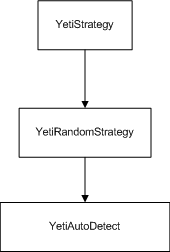
\includegraphics[width=3cm,height=3.5cm]{Hierarchy1.png}
%\caption{Class Hierarchy of automated discovery of failure domains in YETI}
%\label{fig:hierarchy}
%\end{figure}

\subsection{Example}\label{sec:example}
For a concrete example to show how ADFD strategy in YETI proceeds, we suppose YETI tests the following class with ADFD strategy selected for testing. Note that for more clear visibility of the output graph generated by ADFD strategy at the end of test session, we fix the values of lower and upper range by 70 from Integer.MIN\_INT and Integer.MAX\_INT. 

\begin{lstlisting}
/**
 * Point Fault Domain example for one argument
 * @author (Mian and Manuel)
 */
public class PointDomainOneArgument{
	public static void pointErrors (int x){
     		if (x == -66)
       			abort();
     
     		if (x == -2)
     			abort();
      				
     		if (x == 51)
     			abort();
     
     		if (x == 23)
     			abort();
	}
}
\end{lstlisting}

%Published programs from literature \cite{Chen2003}\cite{Chan1996}\cite{Chen2004} of point, block and strip failure patterns are tested to explain the working of ADFD . These programs were translated in to java language for this experiment (See appendix 1 for more details). 

\begin{figure}[H]
\centering
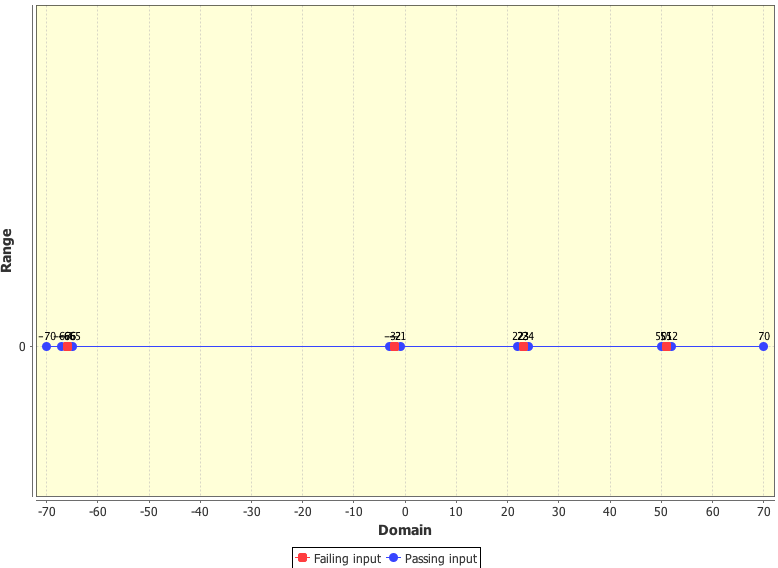
\includegraphics[width=8.2cm,height=3.5cm]{pointDomainOneArgument.png}
\caption{ADFD strategy plotting pass and fault domain of the given class}
\label{fig:ADFD-example}
\end{figure}

As soon as any one of the above four faults are discovered the ADFD strategy generate a dynamic program given in Appendix \ref{sec:appendix1} (1). This program is automatically compiled to get binary file and then executed to find the pass and fail domains inside the specified range. The identified domains are plotted on two-dimensional graph. It is evident from the output presented in Figure \ref{fig:ADFD-example} that ADFD strategy not only finds all the faults but also the pass and fail domains.


\begin{comment}
%%%%%% They are commented in this format to decrease the text, for two column format uncomment them.

ADFD can be activated by typing the command java -jar ADFD.jar. After the GUI of ADFD is launched we need to specify yeti specific values that include language of the program under test, strategy for the current test session, duration of test session (minutes or milli-second), display YETI GUI or not and display real time logs or not. Next we browse to select the file for testing and the run button starts testing the file with YETI tool. 

\begin{figure}[ht]
\centering
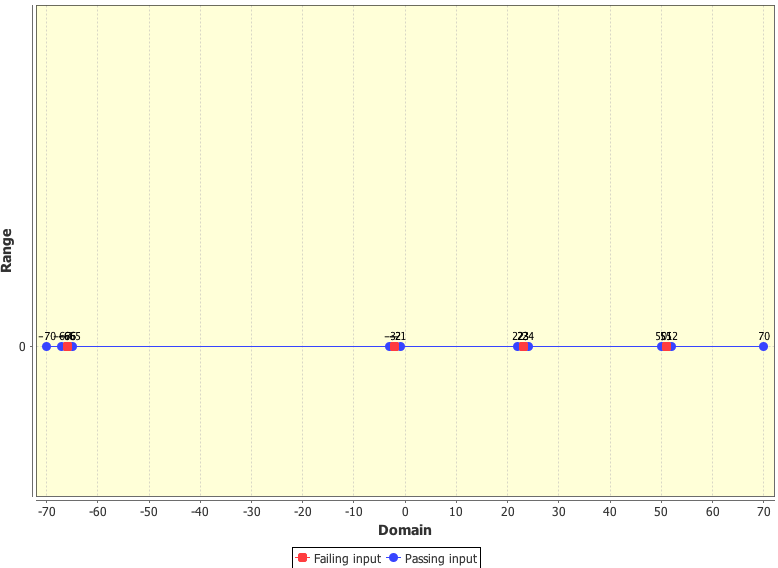
\includegraphics[width=8.2cm,height=5cm]{pointDomainOneArgument.png}
\caption{ADFD strategy plotting pass and fault domain of the given class}
\label{fig:ADFD-example}
\end{figure}

In 5 second YETI found one fault out of the above 4 faults. The ADFD strategy in YETI generate a source file (C*.java) at the end of the test session. This file contain the code that searches for fault domains. The count button count the number of files. ADFD create the number of files on the basis of the number of arguments in the method under test. For one argument one method is created and for two argument two methods are created. 

The next button is compile which compile the generated files and generate the byte code (.class files). The execute button execute the byte code and test the method under test for all the values between upper and lower bound. At the end of execution it generates two files (pass.txt and fail.txt). Pass file contain all the values for which the method performed correctly while fail file contain all the values for which the method under test fail.

The draw fault domain button reads the pass and fail files and plot them on the x, y graph where red line with squares show the failing values while the blue line with square shapes show the passing values.
\end{comment}

%%%%%%%%%%%%%%%%%%%%%%%%%%%%%%%%%%%%%%%%%%%%%%%%%%%%%%%%

\section{Experimental Results} \label{sec:experimentalResults}
This section includes the experimental setup and results obtained after using ADFD strategy. Six numerical programs of one and two-dimension were selected. These programs were error-seeded in such a way to get all the three forms of fault domains including point, block and strip fault domains. Each selected program contained various combinations of one or more fault domains. 

All experiments were performed on a 64-bit Mac OS X Lion Version 10.7.5 running on 2 x 2.66 GHz 6-Core Intel Xeon with 6.00 GB (1333 MHz DDR3) of RAM. YETI runs on top of the Java\texttrademark  SE Runtime Environment [version 1.6.0\_35]. 

To elucidate the results, six programs were developed so as to have separate program for one and two-dimension point, block and strip fault domains. The code of selected programs is given in Appendix \ref{sec:appendix1} (2-7). The experimental results are presented in table \ref{sec:fail table} and described under the following three headings.
%\begin{center}

%\end{center}

\begin{table}[h]
%\renewcommand{\arraystretch}{2}
\centering
\scriptsize
%\normalsize

\begin{tabular}{|c|c|c|l|l|l|}

\hline 


\multirow{2}{*}{S. No}	& \multirow{2}{*}{Fault }	 				& \multirow{2}{*}{Module } 		& \multirow{2}{*}{Specific Fault}	 		& \multirow{2}{*}{Pass Domain} 					& \multirow{2}{*}{Fail Domain} 			\\  
					& Domain								&  Dimension					&									&											&								\\ \hline 
\multirow{6}{*}{1} 	&	\multirow{6}{*}{Point}				& 	\multirow{3}{*}{One}			&	\multirow{3}{*}{PFDOneA(i)}	&	-100 to -67, -65 to -3, 		  		& -66, -2, 23, 51			 	\\  
				&									&							&							&	-1 to 50, 2 to 22, 					&							\\  
				&									&							&							&	24 to 50, 52 to 100					&							\\ \cline{3-6}
				&									&	\multirow{3}{*}{Two}			&	\multirow{2}{*}{PFDTwoA(2, i)}	&	(2, 100) to (2, 1),	 				&  (2, 0)						\\  
				&									&							&							&	(2, -1) to (2, -100)					&							\\ \cline{4-6}
				&									& 							&	PFDTwoA(i, 0)				&	Nil								& (-100, 0) to (100, 0)				\\  \hline



\multirow{5}{*}{2} 	&	\multirow{5}{*}{Block}				& 	\multirow{2}{*}{One}			&	\multirow{2}{*}{BFDOneA(i)}	&	-100 to -30, -25 to -2, 					& 	-1 to 1, -29 to -24,		 	\\ 
				&									&							&							&	2 to 50, 55 to 100						&	51 to 54,				\\   \cline{3-6}
				&									&	\multirow{3}{*}{Two}			&	\multirow{2}{*}{BFDTwoA(-2, i)}	&	(-2, 100) to (-2, 20), 					& 	(-2 , 1) to ( -2, 19), 		\\ 
				&									&							&							&      (-2, -1) to (-2, -100)					&	(-2, 0)				\\ \cline{4-6}
				&									& 							&	BFDTwoA(i, 0)				&	Nil								& 	(-100, 0) to (100, 0)		\\  \hline
				
				



\multirow{5}{*}{3} 	&	\multirow{5}{*}{Strip}					& 	\multirow{2}{*}{One}			&	\multirow{2}{*}{SFDOneA(i)}	&	\multirow{2}{*}{-100 to -5, 35 to 100}		& 	\multirow{2}{*}{-4, 34	}\\ 
				&									&							&							&									&				\\  \cline{3-6}
				&									&	\multirow{3}{*}{Two}			&	\multirow{2}{*}{SFDTwoA(-5, i)}	&	(-5, 100) to (-5, 40),					&  (-5, 39) to (-5, 1), 			\\ 
				&									&							&							&	 (-5, 0) to (-5, -100)					&	(-5, 0)				\\ \cline{4-6}
				&									& 							&	SFDTwoA(i, 0)				&	Nil								&  (-100, 0) to (100, 0)			\\  \hline
				
				
\end{tabular}
\bigskip
\caption{Pass and Fail domain with respect to one and two dimensional program}
\label{tab:failtable}
\end{table}




\noindent \textbf{Point Fault Domain:}  Two separate Java programs Pro2 and Pro3 given in Appendix \ref{sec:appendix1} (2, 3) were tested with ADFD strategy in YETI to get the findings for point fault domain in one and two-dimension program. Figure \ref{fig:PFDOne} present range of pass and fail values for point fault domain in one-dimension whereas Figure \ref{fig:PFDTwo} present range of pass and fail values for point fault domain in two-dimension program. The range of pass and fail values for each program in point fault domain are given in (Table \ref{tab:failtable}, Serial No. 1).
%%%%%%%%%%%%%%%%Point Domain%%%%%%%%%%%%%%%%%%%%%%%%%%%%%

\begin{figure} [H]

\subfigure[One dimension module]{
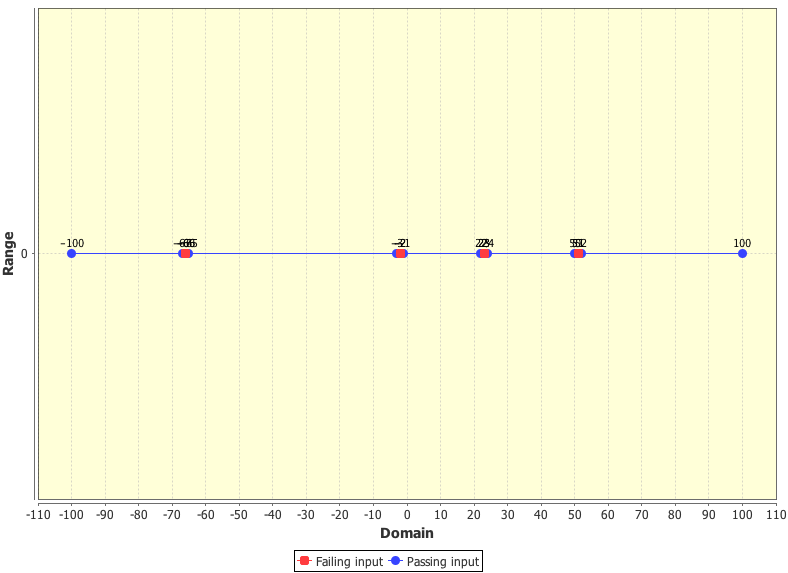
\includegraphics[width=6cm,height=4cm]{PFDOne.png}
\label{fig:PFDOne}
}
\subfigure[Two dimension module]{
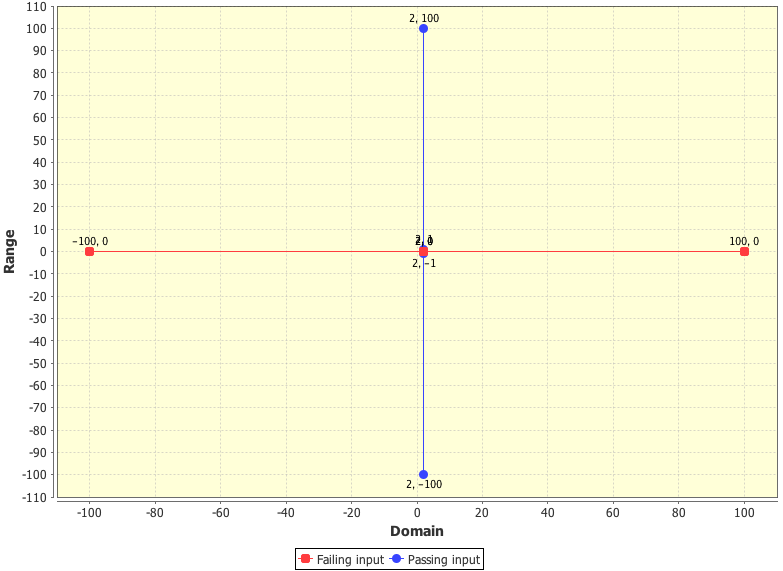
\includegraphics[width=6cm,height=4cm]{PFDTwo.png}
\label{fig:PFDTwo}
}


\caption{Chart generated by ADFD strategy presenting point fault domain}
\end{figure}

%\begin{figure}[H]
%\centering
%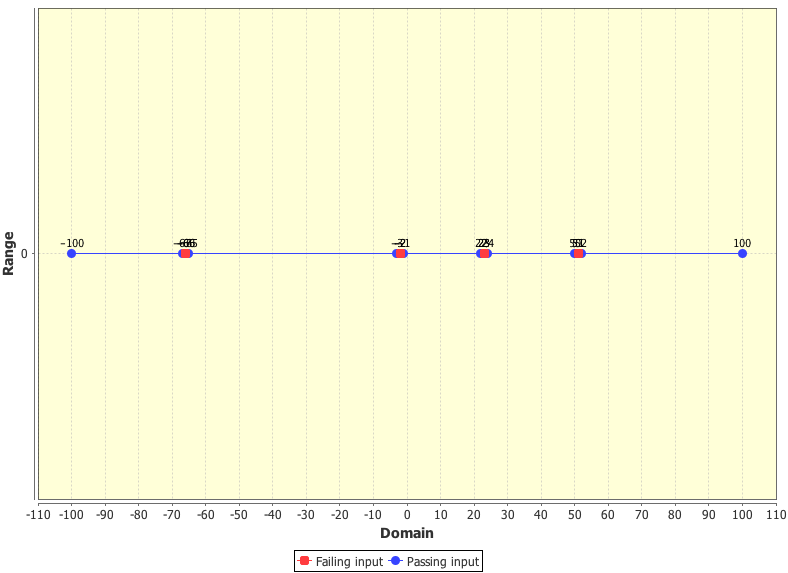
\includegraphics[width=8.2cm,height=5cm]{PFDOne.png}
%\caption{Chart generated by ADFD strategy presenting point fault domain in one dimension module}
%\label{fig:PFDOne}
%\end{figure}

%\begin{figure}[H]
%\centering
%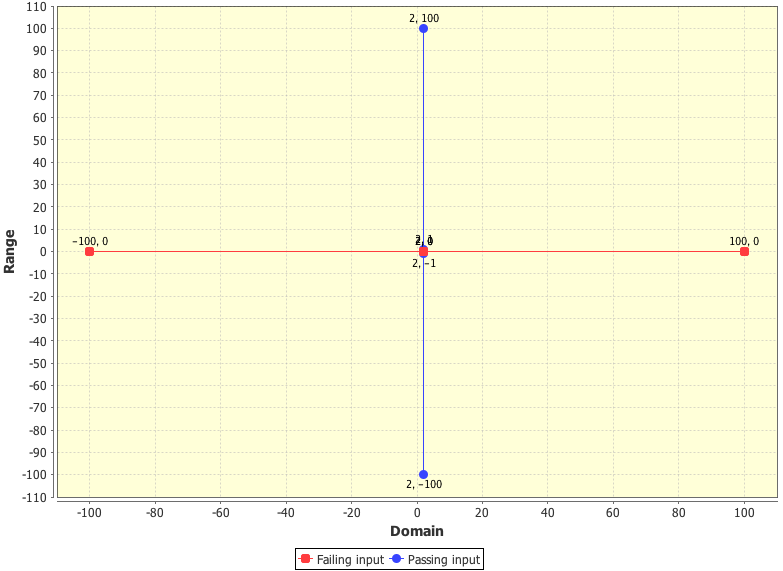
\includegraphics[width=8.2cm,height=5cm]{PFDTwo.png}
%\caption{Chart generated by ADFD strategy presenting point fault domain in two dimension module}
%\label{fig:PFDTwo}
%\end{figure}


\noindent \textbf{Block Fault Domain:}  Two separate Java programs Pro4 and Pro5 given in Appendix \ref{sec:appendix1} (4, 5) were tested with ADFD strategy in YETI to get the findings for block fault domain in one and two-dimension program. Figure \ref{fig:BFDOne} present range of pass and fail values for block fault domain in one-dimension whereas Figure \ref{fig:BFDTwo} present range of pass and fail values for block fault domain in two-dimension program. The range of pass and fail values for each program in block fault domain are given in (Table \ref{tab:failtable}, Serial No. 2).
%%%%%%%%%%%%%%%Block domain %%%%%%%%%%%%%%%%%%%%%%%%%%%%%%
%%%





\begin{figure} [H]

\subfigure[One dimension module]{
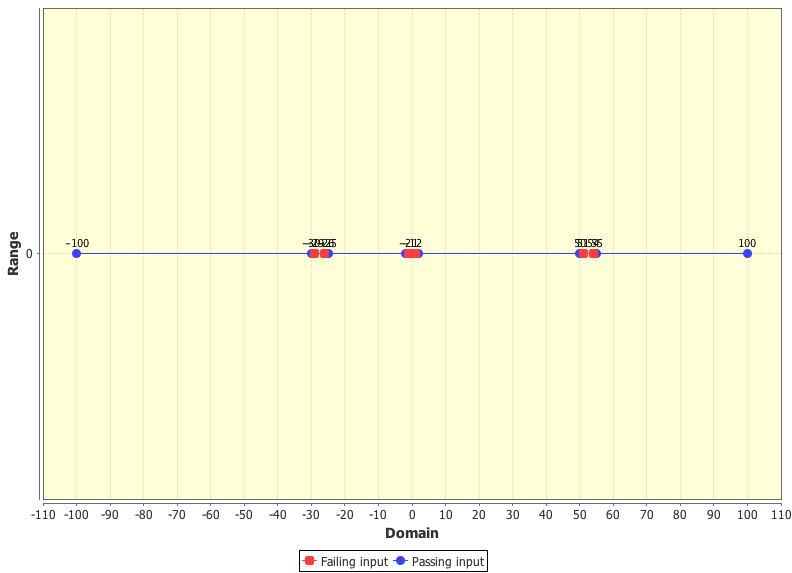
\includegraphics[width=6cm,height=4cm]{BFDOne.png}
\label{fig:BFDOne}
}
\subfigure[Two dimension module]{
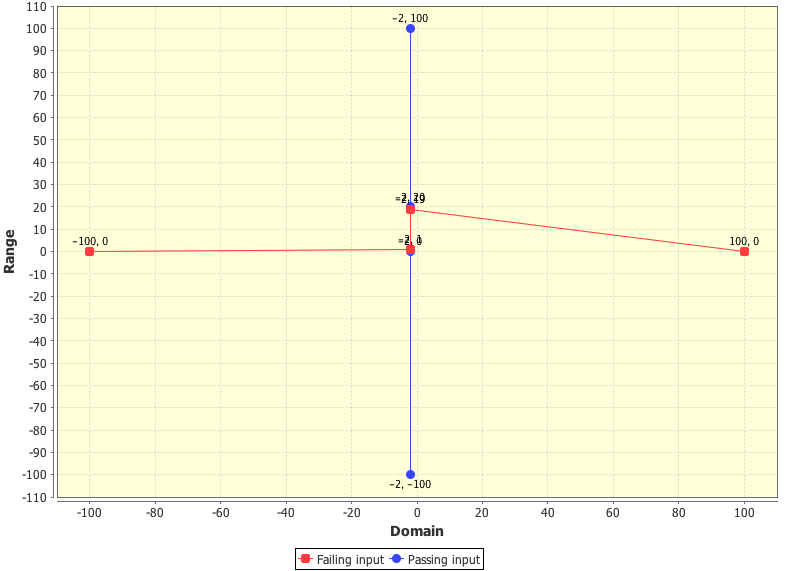
\includegraphics[width=6cm,height=4cm]{BFDTwo.png}
\label{fig:BFDTwo}
}


\caption{Chart generated by ADFD strategy presenting block fault domain}
\end{figure}


%\begin{figure}[H]
%\centering
%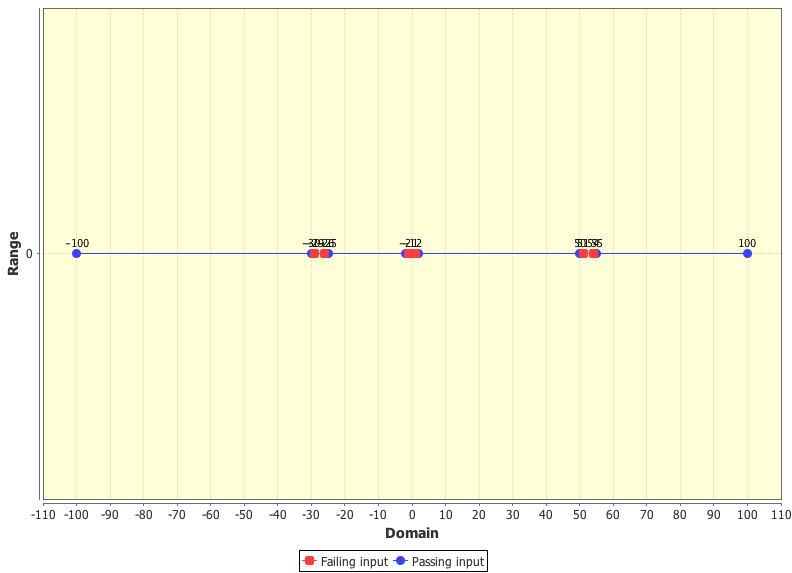
\includegraphics[width=8.2cm,height=5cm]{BFDOne.png}
%\caption{Chart generated by ADFD strategy presenting block fault domain in one dimension module}
%\label{fig:BFDOne}
%\end{figure}


%\begin{figure}[H]
%\centering
%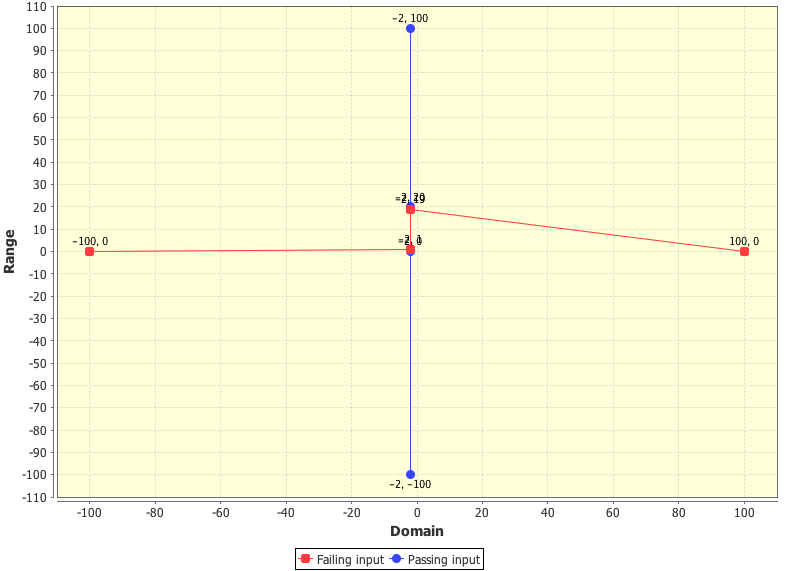
\includegraphics[width=8.2cm,height=5cm]{BFDTwo.png}
%\caption{Chart generated by ADFD strategy presenting block fault domain in two dimension module}
%\label{fig:BFDTwo}
%\end{figure}



\noindent \textbf{Strip Fault Domain:} Two separate Java programs Pro6 and Pro7 given in Appendix \ref{sec:appendix1} (6, 7) were tested with ADFD strategy in YETI to get the findings for strip fault domain in one and two-dimension program. Figure \ref{fig:SFDOne} present range of pass and fail values for strip fault domain in one-dimension whereas Figure \ref{fig:SFDTwo} present range of pass and fail values for strip fault domain in two-dimension program. The range of pass and fail values for each program in strip fault domain are given in (Table \ref{tab:failtable}, Serial No. 3).


%
%%%%%%%%%%%%%%%%%%%%%%Strip domain %%%%%%%%%%%%%%%%%%%%%%%
\begin{figure} [H]

\subfigure[One dimension module]{
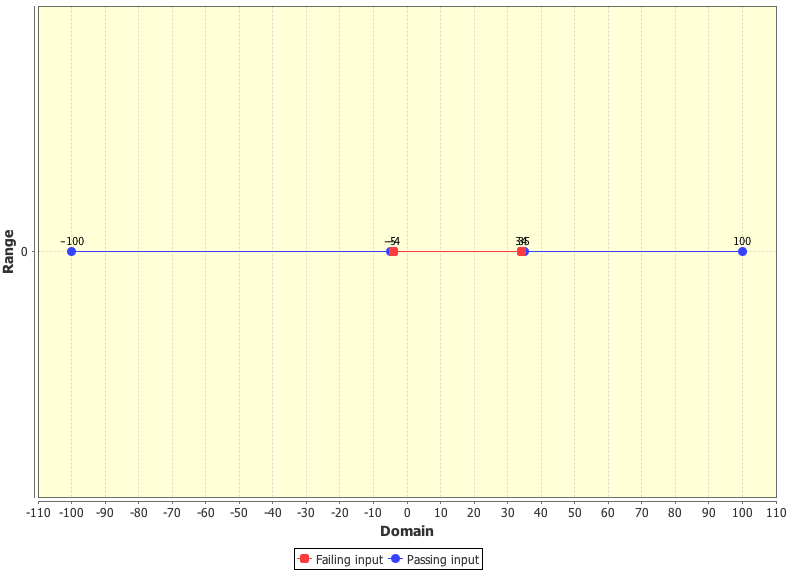
\includegraphics[width=6cm,height=4cm]{SFDOne.png}
\label{fig:SFDOne}
}
\subfigure[Two dimension module]{
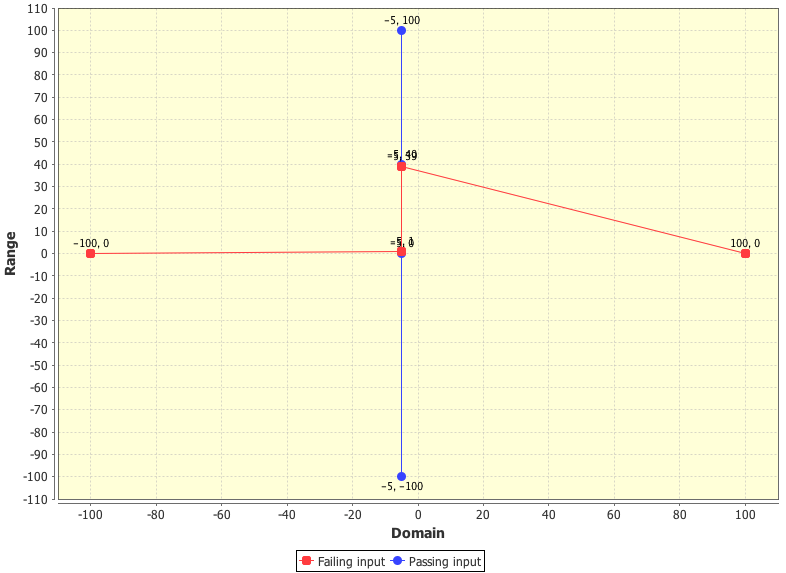
\includegraphics[width=6cm,height=4cm]{SFDTwo.png}
\label{fig:SFDTwo}
}


\caption{Chart generated by ADFD strategy presenting Strip fault domain}
\end{figure}






%\begin{figure}[H]
%\centering
%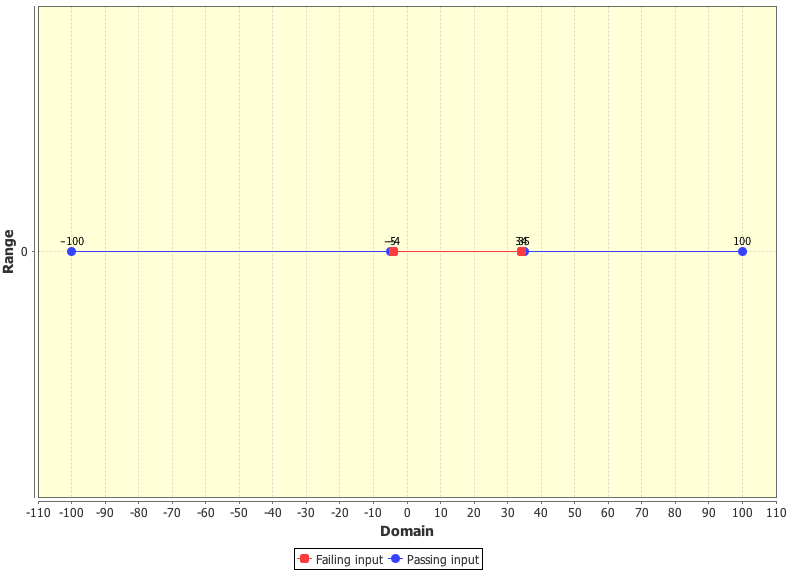
\includegraphics[width=8.2cm,height=5cm]{SFDOne.png}
%\caption{Chart generated by ADFD strategy presenting strip fault domain in one dimension module}
%\label{fig:SFDOne}
%\end{figure}

%\begin{figure}[H]
%\centering
%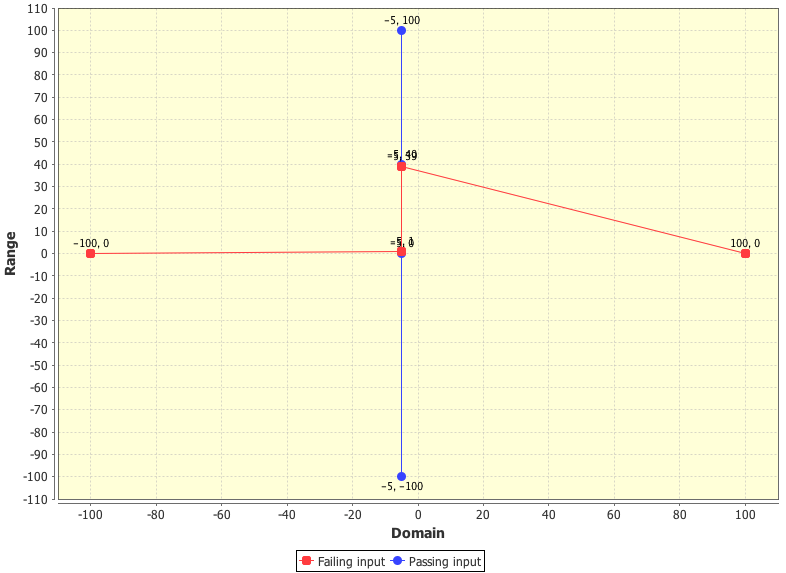
\includegraphics[width=8.2cm,height=5cm]{SFDTwo.png}
%\caption{Chart generated by ADFD strategy presenting strip fault domain in two dimension module}
%\label{fig:SFDTwo}
%\end{figure}



\section{Discussion} \label{sec:discussion}

ADFD strategy with a simple graphical user interface is a fully automated process to identify and plot the pass and fault domains on the chart. Since the default settings are all set to optimum the user needs only to specify the module to be tested and click ``Draw fault domain" button to start test execution. All the steps including Identification of fault, generation of dynamic java program to find domain of the identified fault, saving the program to a permanent media, compiling the program to get its binary, execution of binaries to get pass and fail domain and plotting these values on the graph are done completely automated without any human intervention.

In the experiments (section \ref{sec:experimentalResults}), the ADFD strategy effectively identified faults and faults domain in a program. Identification of fault domain is simple for one and two dimension numerical program but the difficulty increases as the program dimension increases beyond two. Similarly no clear boundaries are defined for non-numerical data therefore it is not possible to plot domains for non-numerical data unless some boundary criteria is defined.

ADFD strategy initiate testing with random+ strategy to find the fault and later switch to brute-force strategy to apply all the values between upper and lower bound for finding pass and fault domain. 
It is found that faults at boundary of the input domain can pass unnoticed through ordinary random test strategy but not from ADFD strategy as it scan all the values between lower and upper range.


The overhead in terms of execution time associated with ADFD strategy is dependent mainly on the lower and upper bound. If the lower and upper bound is set to maximum range (i.e. minimum for int is Integer.MIN\_INT and maximum Integer.MAX\_INT) then the test duration is maximum. It is rightly so because for identification of fault domain the program is executed for every input available in the specified range. Similarly increasing the range also shrinks the produced graph making it difficult to identify clearly point, block and strip domain unless they are of considerable size. Beside range factor, test duration is also influenced by the identification of the fault and the complexity of module under test.

ADFD strategy can help the debuggers in two ways. First, it reduces the to and from movement of the project between the testers and debuggers as it identity all the faults in one go. Second, it identifies locations of all fault domains across the input domain in a user-friendly way helping debugger to fix the fault keeping in view its all occurrences.


\section{Threats to Validity} \label{sec:validity}
The major external threat to the use of ADFD strategy on commercial scale is the selection of small set of error-seeded programs of only primitive types such as integer used in the experiments. However, the present study will serve as foundation for future work to expand it to general-purpose real world production application containing scalar and non-scalar data types.

Another issue is the easy plotting of numerical data in the form of distinctive units, because it is difficult to split the composite objects containing many fields into units for plotting. Some work has been done to quantify composite objects into units on the basis of multiple features\cite{Ciupa2006},to facilitate easy plotting. Plotting composite objects is beyond the scope of the present study. However, further studies are required to look in to the matter in depth. 

Another threat to validity includes evaluating program with complex and more than two input arguments. ADFD strategy has so far only considered scalar data of one and two-dimensions. However, plotting domain of programs with complex non-scalar and more than two dimension argument is much more complicated and needs to be taken up in future studies.

Finally, plotting the range of pass or fail values for a large input domain (Integer.MIN\_INT to Integer.MAX\_INT) is difficult to adjust and does not give a clearly understandable view on the chart. Therefore zoom feature is added to the strategy to zoom into the areas of interest on the chart.



\section{Related Works} \label{sec:relatedWork}
Traditional random testing is quick, easy to implement and free from any bias. In spite of these benefits, the lower fault finding ability of traditional random testing is often criticised \cite{Offutt1996}, \cite{Myers2011}. To overcome the performance issues without compromising on its benefits, various researchers have altered its algorithm as explained in section 1. Most of the alterations are based on the existence of faults and fault domains across the input domain \cite{Chan1996}. 

Identification, classification of pass and fail domains and visualisation of domains have not received due attention of the researchers. Podgurski et. al., \cite{Podgurski2003} proposed a semi-automated procedure to classify similar faults and plot them by using a Hierarchical Multi Dimension Scaling (HMDS) algorithm. A tool named Xslice \cite{Agrawal1995} visually differentiates the execution slices of passing and failing part of a test. Another tool called Tarantula uses colour coding to track the statements of a program during and after the execution of the test suite \cite{Jones2002}. A serious limitation of the above mentioned tools is that they are not fully automated and require human interaction during execution. Moreover these tools are based on the already existing test cases where as ADFD strategy generate test cases, discover faults, identify pass and fault domains and visualise them in a fully automated manner. 


\section{Conclusion} \label{sec:conclusion}

Results of the experiments (section 4), based on applying ADFD strategy to error-seeded numerical programs provide, evidence that the strategy is highly effective in identifying the faults and plotting pass and fail domains of a given SUT. It further suggests that the strategy may prove effective for large programs. However, it must be confirmed with programs of more than two-dimension and different non-scalar argument types. ADFD strategy can find boundary faults quickly as against the traditional random testing, which is either, unable or takes comparatively long time to discover the faults.

The use of ADFD strategy is highly effective in testing and debugging. It provides an easy to understand test report visualising pass and fail domains. It reduces the number of switches of SUT between testers and debuggers because all the faults are identified after a single execution. It improves debugging efficiency as the debuggers keep all the instances of a fault under consideration when debugging the fault.


\bigskip
%ACKNOWLEDGMENTS are optional
\noindent\textbf{Acknowledgments} \\*

The authors thank the Department of Computer Science, University of York for its financial support with the Departmental Overseas Research Scholarship (DORS) award. We also thanks to Richard Page for his valuable help and generous support.


























\section{The References Section}
\renewcommand\refname{}
\vspace*{-0.7cm}
\bibliographystyle{splncs}
\bibliography{sigproc}












\section*{Appendix:} \label{sec:appendix1}
\scriptsize


\textbf{Program 1} Program generated by ADFD on finding fault in SUT
\begin{lstlisting}
/**
 * Dynamically generated code by ADFD strategy 
 * after a fault is found in the SUT.
 * @author (Mian and Manuel)
 */
import java.io.*;
import java.util.*;

public class C0 
{
	public static ArrayList<Integer> pass = new ArrayList<Integer>();
	public static ArrayList<Integer> fail = new ArrayList<Integer>();
	public static boolean startedByFailing = false;
	public static boolean isCurrentlyFailing = false;
	public static int start = -80; 
	public static int stop = 80;

	public static void main(String []argv){
		checkStartAndStopValue(start);
		for (int i=start+1;i<stop;i++){
			try{
				PointDomainOneArgument.pointErrors(i);
				if (isCurrentlyFailing) 
				{
					fail.add(i-1);
					fail.add(0);
					pass.add(i);
					pass.add(0);
					isCurrentlyFailing=false; 
				} 
			} 
			catch(Throwable t) { 
				if (!isCurrentlyFailing) 
				{
					pass.add(i-1);
					pass.add(0);
					fail.add(i);
					fail.add(0);
					isCurrentlyFailing = true;
				}  
			} 
		} 
		checkStartAndStopValue(stop); 
		printRangeFail(); 
		printRangePass();  
	}

	public static void printRangeFail() { 
		try { 
			File fw = new File("Fail.txt"); 
			if (fw.exists() == false) { 
				fw.createNewFile(); 
			}
			PrintWriter pw = new PrintWriter(new FileWriter (fw, true));   
			for (Integer i1 : fail) { 
				pw.append(i1+"\n"); 
			} 
			pw.close(); 
		} 
		catch(Exception e) { 
			System.err.println(" Error : e.getMessage() "); 
		} 
	} 
	public static void printRangePass() { 
		try { 
			File fw1 = new File("Pass.txt"); 
			if (fw1.exists() == false) { 
				fw1.createNewFile(); 
			}
			PrintWriter pw1 = new PrintWriter(new FileWriter (fw1, true));   
			for (Integer i2 : pass) { 
				pw1.append(i2+"\n");
			} 
			pw1.close(); 
		} 
		catch(Exception e) { 
			System.err.println(" Error : e.getMessage() "); 
		} 
	} 
	public static void checkStartAndStopValue(int i) { 
		try { 
			PointDomainOneArgument.pointErrors(i);
			pass.add(i); 
			pass.add(0);
		} 
		catch (Throwable t) { 
			startedByFailing = true; 
			isCurrentlyFailing = true; 
			fail.add(i); 
			fail.add(0);
		} 
	} 
}

\end{lstlisting}


%%%%%%%%%%%%%%%%%%%%%%%%%%%%%%%%%%%%%%%%%%%%%%%%%%%%%%%%%%%%%%%%%%%%%%%%%%%%%%%%%%%%%%%%%%%%%%
\textbf{Program 2} Point domain with One argument
\begin{lstlisting} 
/**
 * Point Fault Domain example for one argument
 * @author (Mian and Manuel)
 */
public class PointDomainOneArgument{

	public static void pointErrors (int x){
		if (x == -66 )
			x = 5/0;

		if (x == -2 )
			x = 5/0;

		if (x == 51 )
			x = 5/0;

		if (x == 23 )
			x = 5/0;
	}
}
\end{lstlisting}
%%%%%%%%%%%%%%%%%%%%%%%%%%%%%%%%%%%%%%%%%%%%%%%%%%%%%%%%%%%%%%%%%%%%%%%%%%%%%%%%%%%%%%%%%%%%%%
\textbf{Program 3} Point domain with two argument
\begin{lstlisting}
/**
 * Point Fault Domain example for two arguments
 * @author (Mian and Manuel)
 */
public class PointDomainOneArgument{

	public static void pointErrors (int x, int y){
		int z = x/y;
	}

}
\end{lstlisting}

%%%%%%%%%%%%%%%%%%%%%%%%%%%%%%%%%%%%%%%%%%%%%%%%%%%%%%%%%%%%%%%%%%%%%%%%%%%%%%%%%%%%%%%%%%%%%%
\textbf{Program 4} Block domain with one argument
\begin{lstlisting}
/**
 * Block Fault Domain example for one arguments
 * @author (Mian and Manuel)
 */

public class BlockDomainOneArgument{

public static void blockErrors (int x){
	
	if((x > -2) \&\& (x < 2))
		x = 5/0;
	
	if((x > -30) \&\& (x < -25))
		x = 5/0;
	
	if((x > 50) \&\& (x < 55))
		x = 5/0;

   }
}

\end{lstlisting}
%%%%%%%%%%%%%%%%%%%%%%%%%%%%%%%%%%%%%%%%%%%%%%%%%%%%%%%%%%%%%%%%%%%%%%%%%%%%%%%%%%%%%%%%%%%%%%
\textbf{Program 5} Block domain with two argument
\begin{lstlisting}
/**
 * Block Fault Domain example for two arguments
 * @author (Mian and Manuel)
 */
public class BlockDomainTwoArgument{

	public static void pointErrors (int x, int y){

		if(((x > 0)\&\&(x < 20)) || ((y > 0) \&\& (y < 20))){
		x = 5/0;
		}
  	
	}

}
\end{lstlisting}
%%%%%%%%%%%%%%%%%%%%%%%%%%%%%%%%%%%%%%%%%%%%%%%%%%%%%%%%%%%%%%%%%%%%%%%%%%%%%%%%%%%%%%%%%%%%%%

\textbf{Program 6} Strip domain with One argument
\begin{lstlisting}
/**
 * Strip Fault Domain example for one argument
 * @author (Mian and Manuel)
 */

public class StripDomainOneArgument{

	public static void stripErrors (int x){
	
		if((x > -5) \&\& (x < 35))
			x = 5/0;
  	 }
}
\end{lstlisting}
%%%%%%%%%%%%%%%%%%%%%%%%%%%%%%%%%%%%%%%%%%%%%%%%%%%%%%%%%%%%%%%%%%%%%%%%%%%%%%%%%%%%%%%%%%%%%%
\textbf{Program 7} Strip domain with two argument
\begin{lstlisting}
/**
 * Strip Fault Domain example for two arguments
 * @author (Mian and Manuel)
 */
public class StripDomainTwoArgument{

	public static void pointErrors (int x, int y){

		if(((x > 0)\&\&(x < 40)) || ((y > 0) \&\& (y < 40))){
		x = 5/0;
		}
  	
	}

}

\end{lstlisting}
%%%%%%%%%%%%%%%%%%%%%%%%%%%%%%%%%%%%%%%%%%%%%%%%%%%%%%%%%%%%%%%%%%%%%%%%%%%%%%%%%%%%%%%%%%%%%%



\end{document}
